\documentclass[12pt, a4]{article}
\usepackage[english]{babel}
\usepackage[utf8]{inputenc}
\usepackage{fullpage}
\usepackage{listings}
\usepackage{graphicx}
\usepackage{color}

%Syntax highlighting
\definecolor{blue-violet}{rgb}{0.54, 0.17, 0.89}
\definecolor{ao}{rgb}{0.0, 0.5, 0.0}
\definecolor{amaranth}{rgb}{0.9, 0.17, 0.31}
\definecolor{ballblue}{rgb}{0.13, 0.67, 0.8}
\definecolor{onyx}{rgb}{0.06, 0.06, 0.06}


\lstset{
  breaklines=true,                 % automatic line breaking only at whitespace
  captionpos=b,                    % sets the caption-position to bottom
  breakatwhitespace=false,
  keepspaces=true,
  numbers=left,
  numbersep=5pt,
  showspaces=false,
  showstringspaces=false,
  showtabs=false,
  tabsize=4,  
  backgroundcolor=\color{white},   % choose the background color
  commentstyle=\color{ao},    % comment style
  keywordstyle=\color{amaranth},    % keyword style
  stringstyle=\color{blue-violet},    % string literal style
  numberstyle=\tiny\color{ballblue},	   % number style
  basicstyle=\ttfamily\footnotesize\color{onyx} % size of fonts used for the code
}


%Document Header
\title{\textbf{Department of CSE\\SSN College of Engineering}}
\author{\textbf{Vishakan Subramanian - 18 5001 196 - Semester VI}}
\date{11 April 2021}

\begin{document}
\maketitle
\hrule
\section*{\center{UCS 1611 - Internet Programming Lab}}
\hrule
\bigskip

%Assignment Details
\subsection*{\center{\textbf{Exercise 5: Profile Servlet Using Session and MySQL}}}
\subsection*{\flushleft{Learning Objective:}}
\begin{flushleft}
Implement Profile Servlet using Http Sessions. The specifications are given below.

\begin{enumerate}
\item The login page should contain username, password, login button and
logout button. On clicking login button, invoke the LoginServlet.
\item The LoginServlet should authenticate the user and store the username in
session for viewing his profile and display a message “Welcome username”. 
\item The LoginServlet should also display a link “View Profile in Detail”. The link when clicked, should invoke ProfileServlet.
\item ProfileServlet should display the username retrieved from the session with the message “Welcome username to the profile page”. Also retrieve and
display the detail information of the user from the database in that page. It
also displays a link to the Login page to logout.
\item When Logout button is pressed, invoke the LogoutServlet. 
\item LogoutServlet should invalidate the user session and display “Successfully Logged out”.
\end{enumerate}
 
\end{flushleft}

%Code
\newpage
\subsection*{\flushleft{Code - Login HTML:}}
\begin{flushleft}
\lstinputlisting[language = HTML]{profile/index.html}
\end{flushleft}

\newpage
\subsection*{\flushleft{Code - CSS Code:}}
\begin{flushleft}
\lstinputlisting[language = HTML]{profile/styles.css}
\end{flushleft}

\subsection*{\flushleft{Code - Logout JavaScript:}}
\begin{flushleft}
\lstinputlisting[language = Java]{profile/scripts/logout.js}
\end{flushleft}

\newpage
\subsection*{\flushleft{Code - Web XML:}}
\begin{flushleft}
\lstinputlisting[language = XML]{profile/WEB-INF/web.xml}
\end{flushleft}

\newpage
\subsection*{\flushleft{Code - Login Servlet:}}
\begin{flushleft}
\lstinputlisting[language = Java]{profile/Servlets/LoginServlet.java}
\end{flushleft}

\newpage
\subsection*{\flushleft{Code - Profile Servlet:}}
\begin{flushleft}
\lstinputlisting[language = Java]{profile/Servlets/ProfileServlet.java}
\end{flushleft}

\newpage
\subsection*{\flushleft{Code - Logout Servlet:}}
\begin{flushleft}
\lstinputlisting[language = Java]{profile/Servlets/LogoutServlet.java}
\end{flushleft}

\newpage
\subsection*{\flushleft{Code - SQL Script:}}
\begin{flushleft}
\lstinputlisting[language = SQL]{profile/scripts/script.sql}
\end{flushleft}

%Output
\newpage
\subsection*{\flushleft{Output - Login Page:}}
\begin{figure}[h]
\centering
\caption{Browser Output: Login Page.}
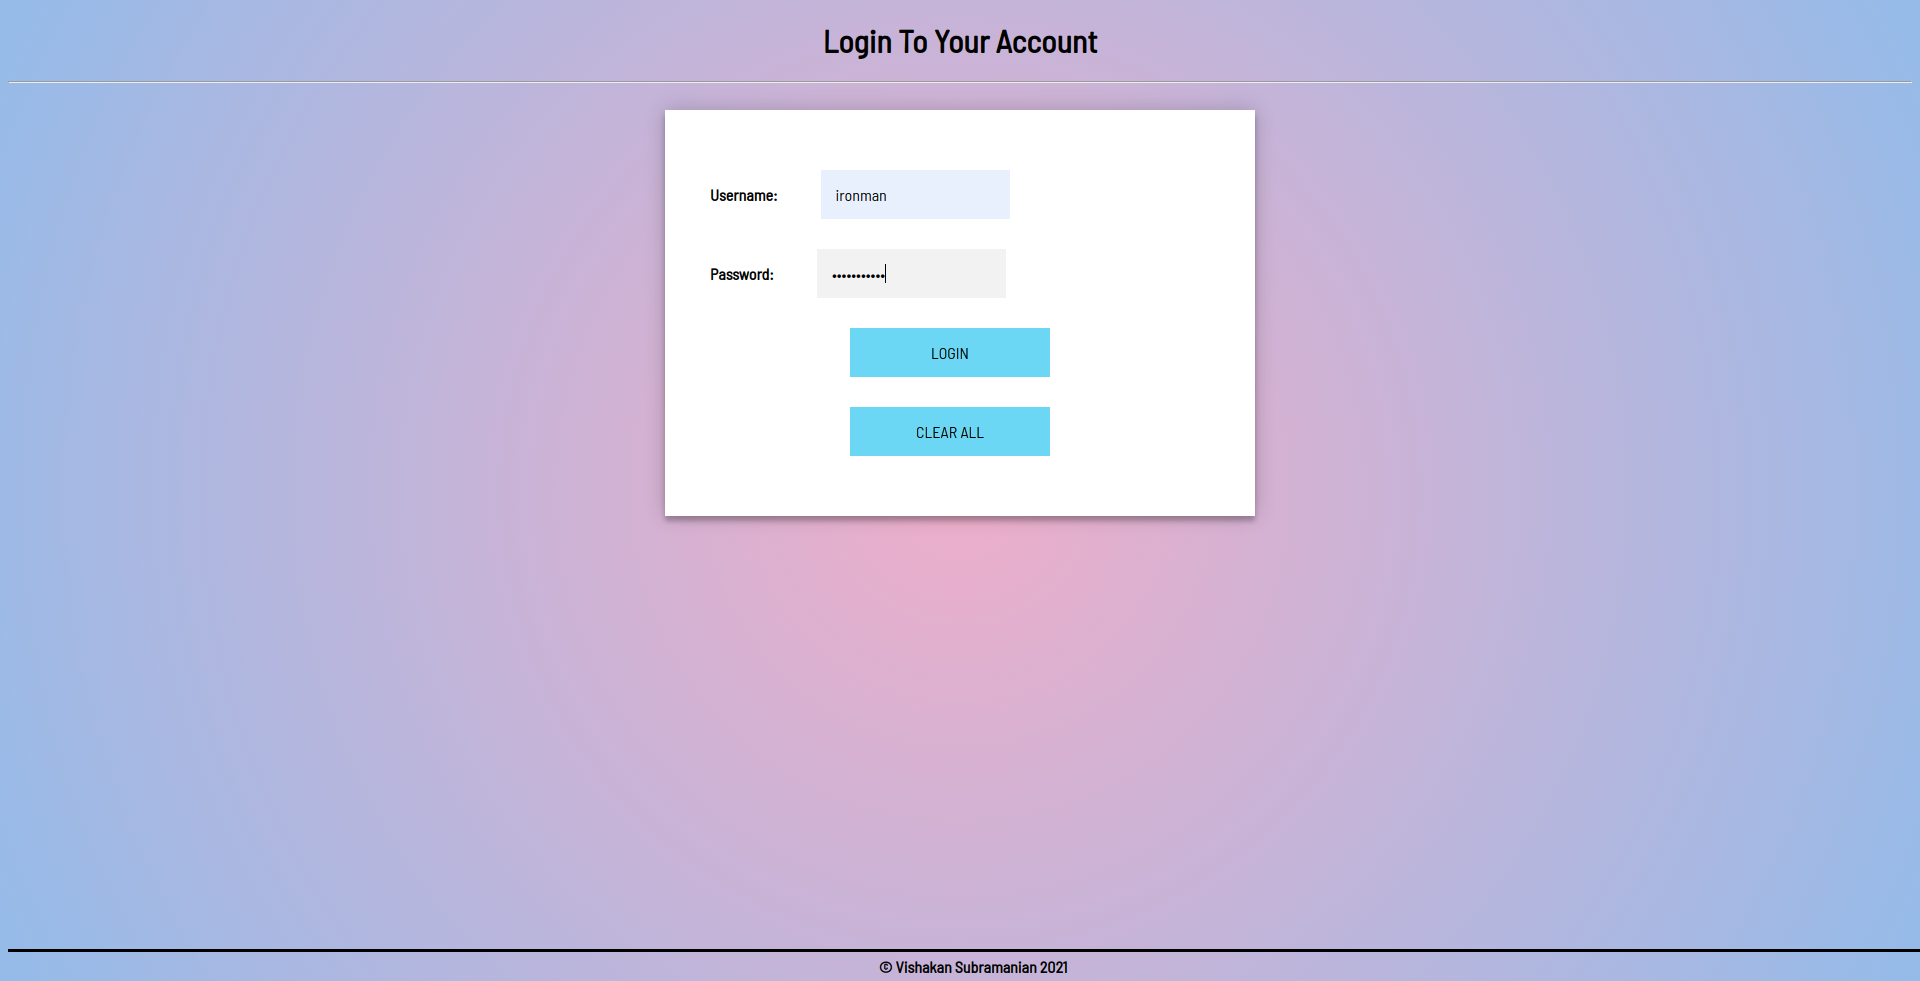
\includegraphics[height=15cm, width=18cm]{Output/Login.png}
\end{figure}

\newpage
\subsection*{\flushleft{Output - Welcome Page:}}
\begin{figure}[h]
\centering
\caption{Browser Output: Welcome Page.}
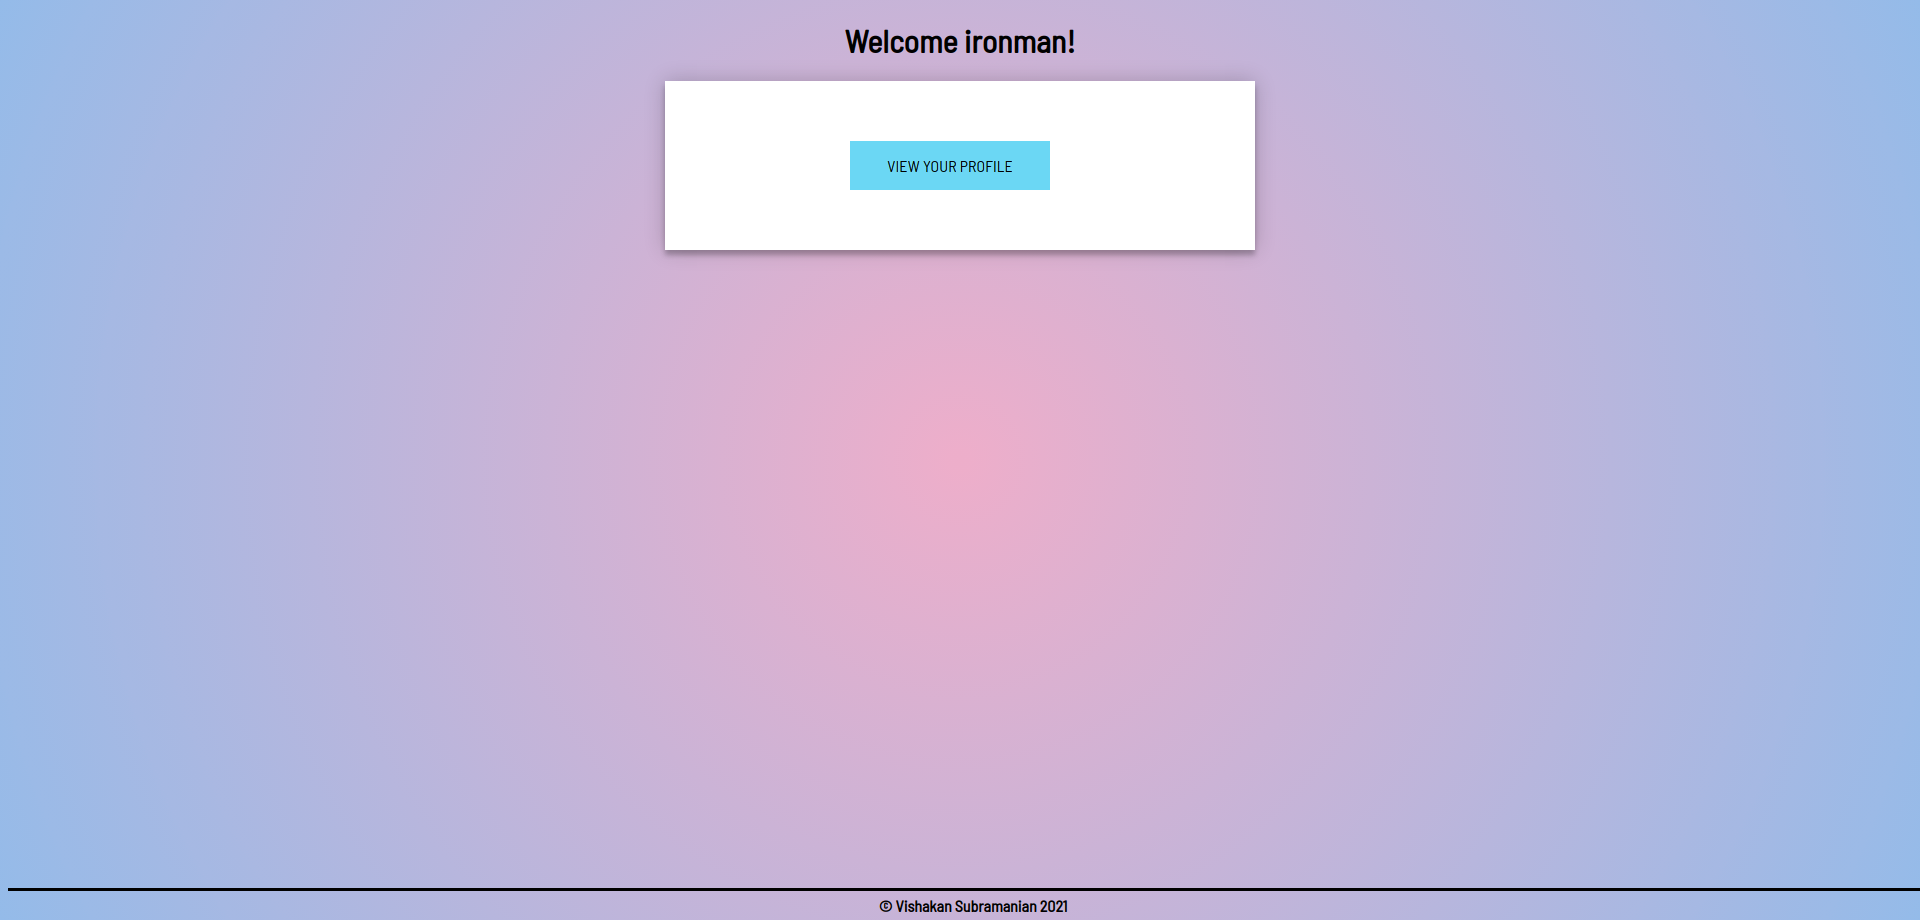
\includegraphics[height=12cm, width=18cm]{Output/Welcome.png}
\end{figure}

\newpage
\subsection*{\flushleft{Output - Profile Page:}}
\begin{figure}[h]
\centering
\caption{Browser Output: Profile Page.}
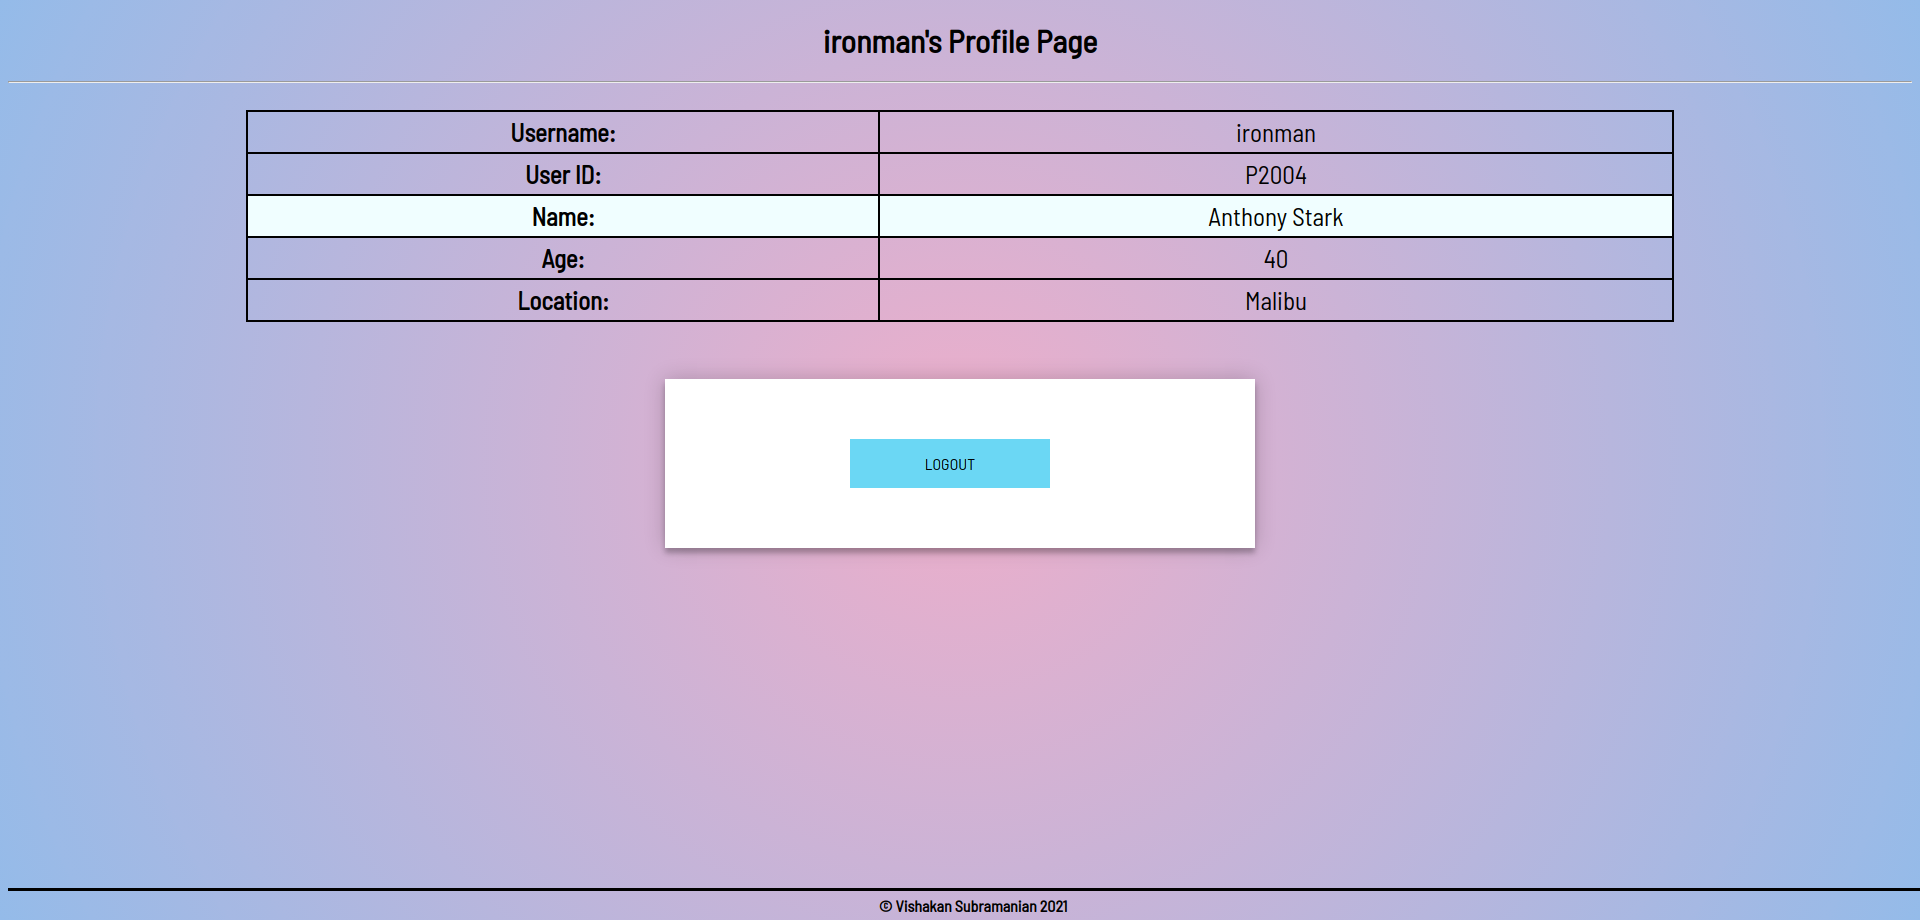
\includegraphics[height=12cm, width=18cm]{Output/Profile.png}
\end{figure}

\newpage
\subsection*{\flushleft{Output - Logout Page:}}
\begin{figure}[h]
\centering
\caption{Browser Output: Logout Page.}
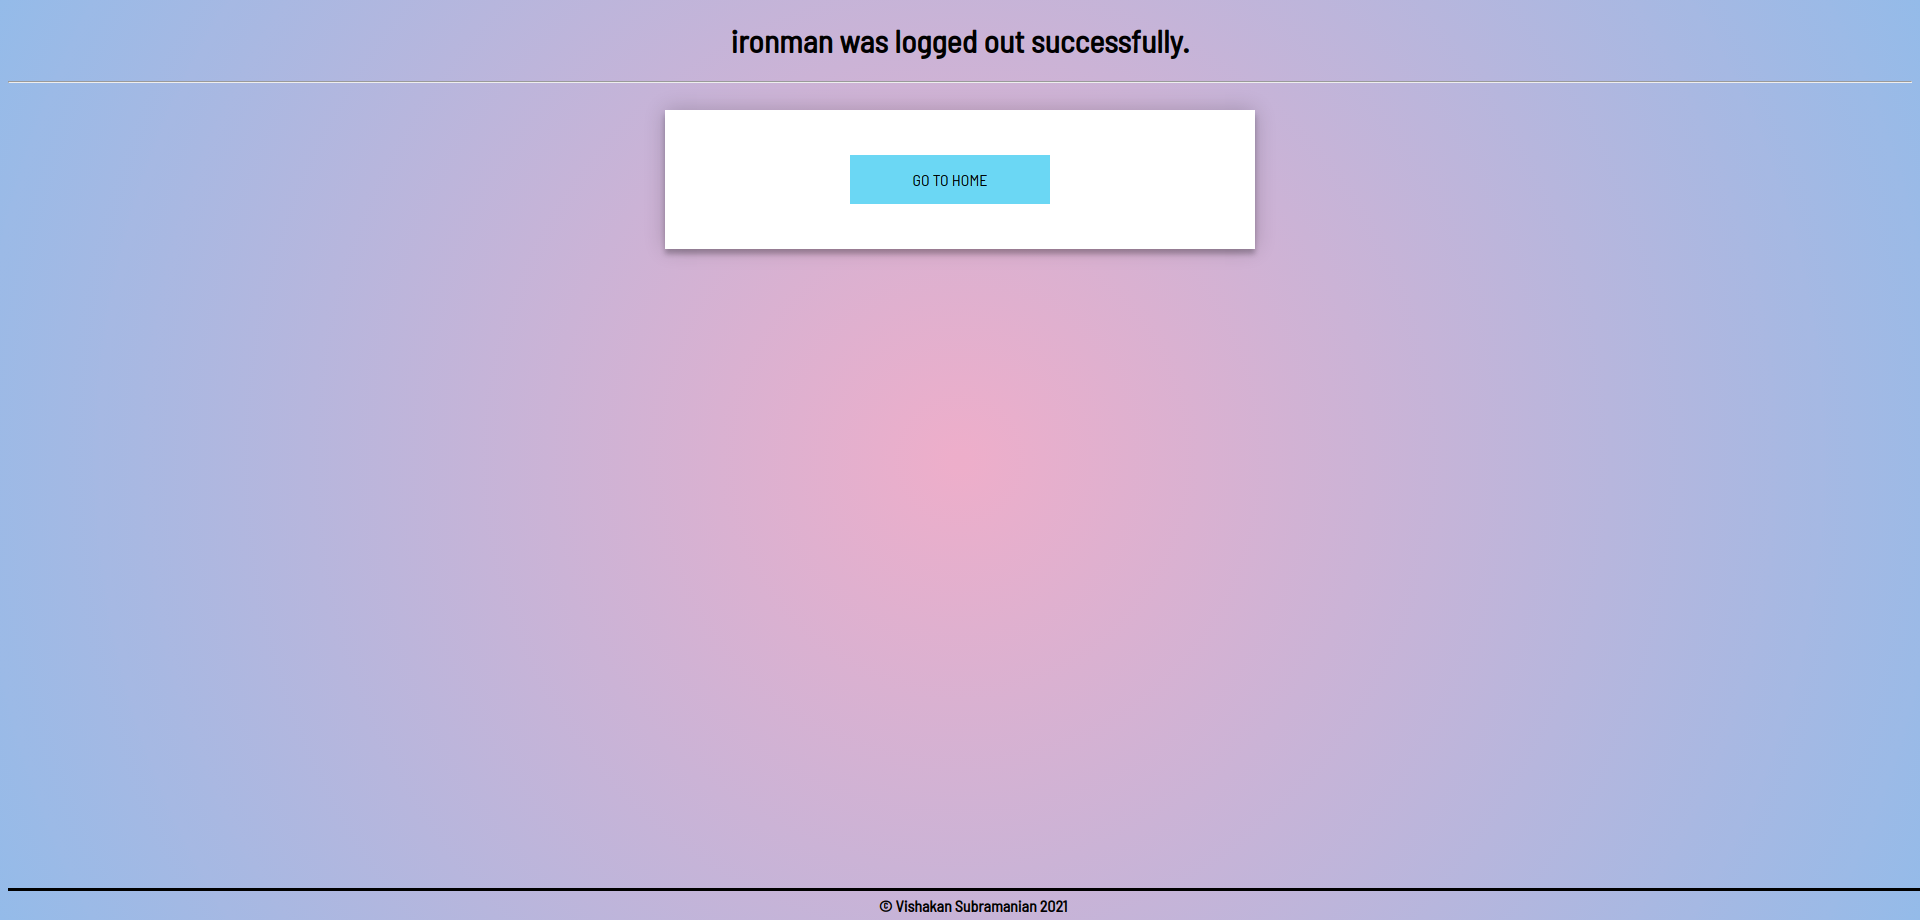
\includegraphics[height=12cm, width=18cm]{Output/Logout.png}
\end{figure}

\newpage
\subsection*{\flushleft{Output - SQL Table:}}
\begin{figure}[h]
\centering
\caption{Browser Output: SQL Table.}
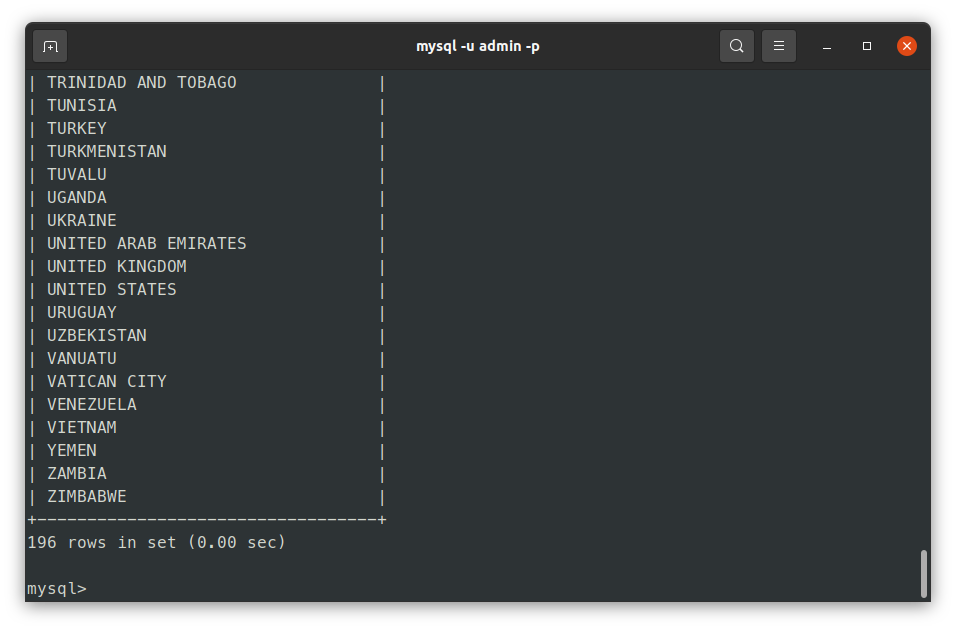
\includegraphics[height=12cm, width=18cm]{Output/SQLTable.png}
\end{figure}

%Learning Outcome
\newpage
\subsection*{\flushleft{Learning Outcome:}}
\begin{itemize}

\item From the experiment, I learnt to implement basic \textbf{Java Servlets}.
\item I learnt about the working of a Java Servlet.
\item I understood that Servlets are executed in the server-side in response to an HTML event like a submit event, and handles actions through a Request-Response mechanism.
\item I was able to serve a dynamic web page using Java Servlet programming.
\item I learnt how to extract HTML Form data from Servlets submitted using the GET query.
\item I was able to create and use a \textbf{HTTPSession} object using server-side Java programming during user login.
\item I used the stored HTTPSession details to retrieve user profile details on user navigation to his/her profile page.
\item I successfully implemented a working \textbf{HTTP Session} using Java Servlet programming and deployed it using the \textbf{Tomcat 9.0 Container}.
\item I refreshed my SQL concepts.
\item I learnt how to integrate MySQL to Java using JDBC Driver.
\item I was able to create a database for User Profiles using MySQL.
\item I successfully implemented JDBC connectivity to MySQL.
\item I implemented credential verification for the login credentials entered by the user in the front-end and verified it with my back-end MySQL storage using a Java Servlet.
\item I learnt to redirect to another page using JavaScript.
\item I understood how to handle basic SQLExceptions with the help of the try-catch block in Java.
\item I understood how to display records dynamically with the help of ResultSet Object in Java and $<$table$>$ element in HTML.
\item I was able to invalidate an HTTPSession on user logout.
\item I was able to successfully implement a working \textbf{Profile Tracking System} according to the given specifications with Java Servlets and MySQL.

\end{itemize}

\end{document}
